\section{Рекуррентные сети и  трансформерные архитектуры}
\subsection{Развитие идей и инструментов обработки последовательностей}
\subsubsection{Энкодер-Декодер архитектура}
Как было подчеркнуто в предыдущей главе, ссылаясь на \cite{RNN_survey}, алгоритмы не инвариантные к длине последовательности выигрывают по многим возможностям. Скрытые Марковские Модели, или кратко СММ, относятся к такому типу алгоритмов. Однако в них состояние модели зависит только от предыдущего, хотя и существуют модификации расширяющие возможности. Рекуррентные архитектуры нейронных сетей с механизмом LSTM (Long Short Term Memory unit - Механизм Короткой Долгосрочной Памяти) предложенным в \cite{LSTM} обладают возможностью сохранять контекст на протяжении обработки всей последовательности. LSTM не является единственной опцией, и даже он имеет множество модификаций, однако так или иначе все рекуррентные сети отдельно обрабатывают каждый токен, но каким-либо образом учитывают информацию о предыдущих. После прохождения по последовательности вложенное представление последнего токена будет обладать информацией о всей последовательности. Более того, такое представление будет обладать все тем же свойством "семантической компактности" как и отображение \ref{w2v}, однако уже в масштабе целого предложения.
Помимо того, что это само по себе очень полезное свойство, на нем основано главное преумещство энкодер-декодерных архитектур на основе рекуррентных операторов.
\newline
\begin{figure}[h]
\caption{Архитектура RNN для seq2seq задачи, развернутая по ходу последовательности}
\centering
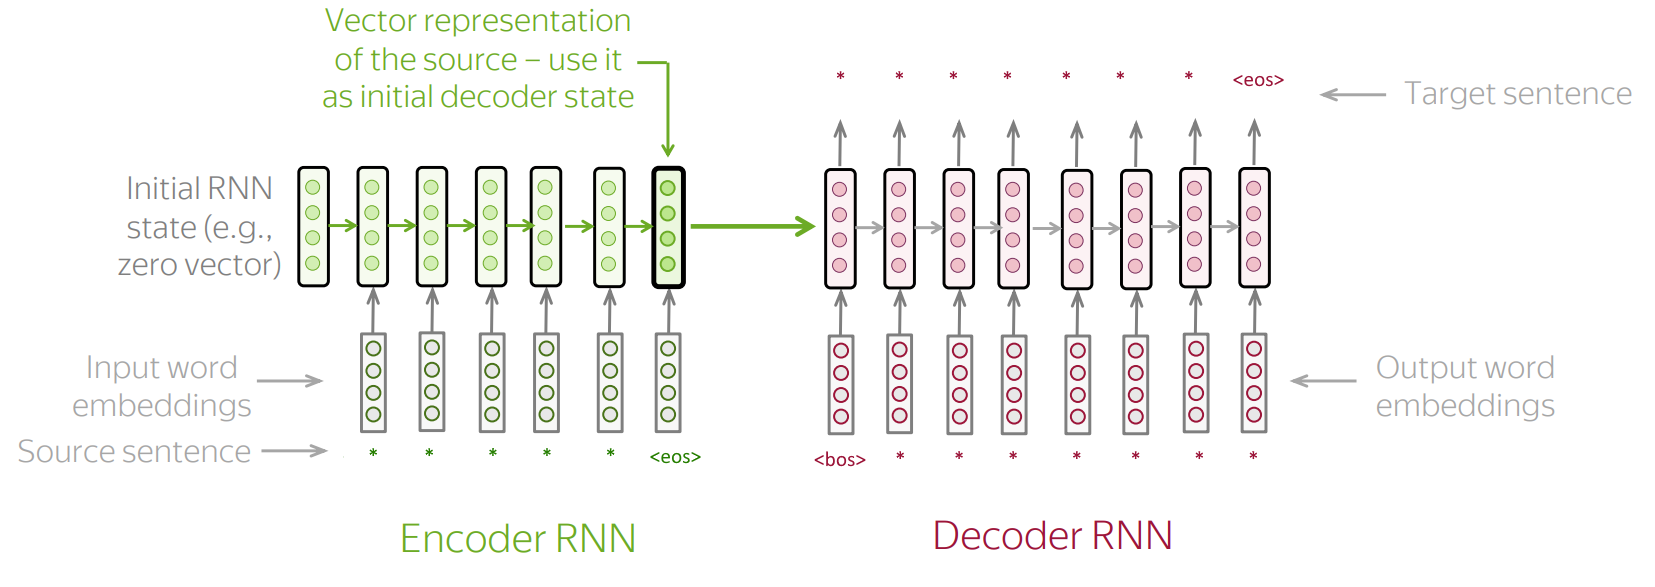
\includegraphics[width=0.75\textwidth]{rnn_arch_base.png}
\label{rnn_arch}
\end{figure}
\newline
Наиболее яркое применение этой архитектуры связано с задачей seq2seq (sequence to sequence или перевод последовательности в последовательность). Последнее соятояние энкодера используется как инициализация для состояний декодера, передавая таким образом информацию для создания новой последовательности извлеченную из входной. Эффективно, это создает "бутылочное горлышко" для сети, заставляя ее наиболее эффективно отражать в этом векторе информацию из последовательности на входе.
\newline
Если задача требует не создан ие новой последовательности, но декодер заменяется на другие операторы, которые будет взаимодействовать как раз таки с последним состоянием последнего слоя энкодера, или его аналогом, как будет показано далее, как с самым информативным и полным представлением об оригинальной последовательности.
\newline
При этом итерация по последовательности может быть как в одну сторону - от начала к концу или наоборот, так и вместе, после чего вложенные преддставления будут сконкатенированны. Такой алгоритм будет называться \textit{Двунаправленным (Bidirectional)}.
% \subsubsection{LSTM}
% \cite{RNN_survey}
\subsubsection{Применение механизма внимания}
Прорывным шагом в работе с энкодер-декодерной архитектурой являлся миханизм внимания\cite{Attention}. Он позволяет не просто использовать последнее состояние энкодера, но управлять тем, какие состояния предыдущего слоя и как использовать, за счет вычисления значимости внимания (Attention Scores) вычислимых между всеми элементами текущей и прошлой последовательностей.
\newline
Гладким аналагом максимума является функция \textit{Softmax}, она и используется для получения значимости внимания:
\begin{equation} \label{softmax} 
\nonumber A \in \mathds{R}^{S}: Softmax(A_{i}) = \frac{A_{i}}_{\sum_{j=1}^{S}exp(A_{j})}
\end{equation}
\textit{Q - Query}, член для которого ведутся вычисления на данном шаге, \textit{K - Key} - все члены последовательности, по которым итеративно идет вычесление, используются для получения значимости внимания между членами; \textit{V - Value} - значение, используемое далее в вычислениях.
Итоговая формула:
\begin{gather} \label{dot_product_att_w/o_scale} 
Attention(Q,K,V) = Softmax \left(QK^{T}\right)V\\
\nonumber \textit{Здесь и далее } d_{k}, d_{v} \in \mathds{N}; Q, K \in \mathds{R}^{d_{k}}, V \in \mathds{R}^{d_{v}}
\end{gather}
Применение механизма внимания отражено на \ref{attn_usg}.

\begin{figure}[h]
\caption{Применение механизма внимания в двунаправленной RNN с MLP - линейными слоями, разделенными активацией-гиперболическим тангенсом,\cite{Attention}}
\centering
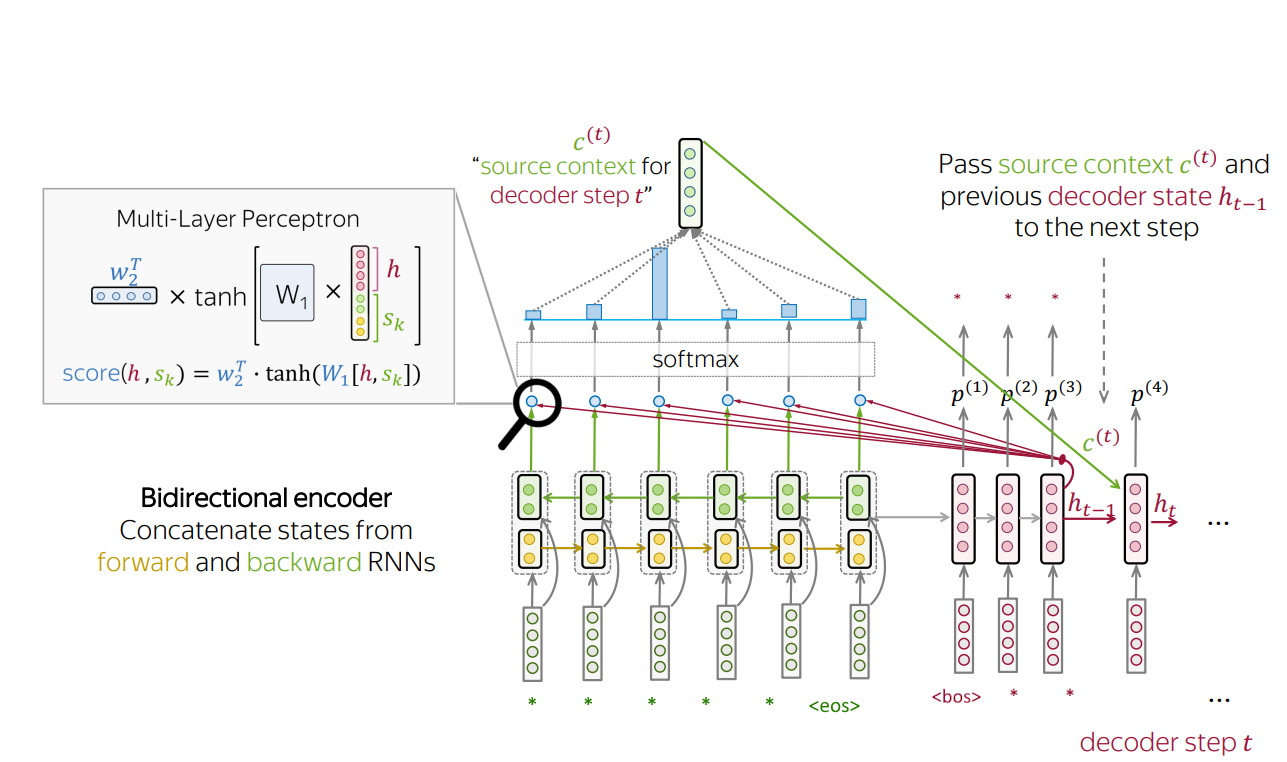
\includegraphics[width=1\textwidth]{attn_usg.png}
\label{attn_usg}
\end{figure}

\subsubsection{Трансформерная архитектура}
В архитектуре трансформерной сети \cite{transformer} нет обычных операторов рекуррентной сети, но используется механизм внимания с множителем для нормализации значений:
\begin{equation} \label{dot_product_att_w/_scale} 
Attention(Q,K,V) = Softmax \left(\frac{QK^{T}}_{\sqrt{d_{k}}}\right)V
\end{equation}
При этом внимание внутри энкодера и декодера применяется с \textit{Q=K=V} и называется \textit{Self-Attention}. Между энкодером и декодером есть связующий мезанизм внимания, где \textit{Q} используется из декодера а \textit{K,V} из энкодера \ref{transformer}.\newline
Так же для больших выразительных способностей внимания, используется версия с множеством голов \textit{h}:
\begin{gather} \label{mh_att} 
\nonumber \textit{}\\
MultiHeadAttention(Q,K,V) = \bigoplus^{h}_{i=0}\left(head_{i}\right)W_{0},\\
\nonumber head_{i} = Attention\left( QW_{i}^{Q},KW_{i}^{K},VW_{i}^{V}\right) - \textit{аналогично \ref{dot_product_att_w/_scale} от линейных }\\ 
\nonumber \textit{комбинаций с собственными весами}
\end{gather}
Наличие разных голов помогает выделять разные типы взаимосвязей между членами последовательности.
\begin{figure}[h]
\caption{Архитектура трансформера}
\centering
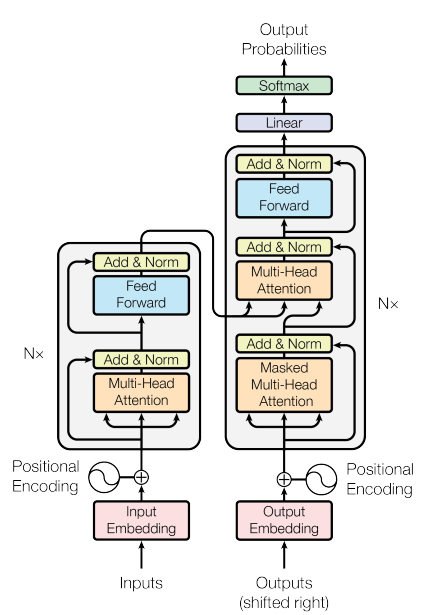
\includegraphics[width=0.37\textwidth]{transformer.png}
\label{transformer}
\end{figure}
\subsection{Технология обучения BERT}
Наиболее мощная претренерованная модель трансформера представлена в \cite{bert}. 
При токенизации добавляются специальные сегментационные токены \textit{[CLS]} и \textit{[SEP]}; первый ставится в начале последовательности, второй отделяет значимые части при работе сразу с двумя последовательностями для задачи с ответом на вопрос (где и разделяетответ и вопрос).
\begin{figure}[h]
\caption{Токенизация в BERT}
\centering
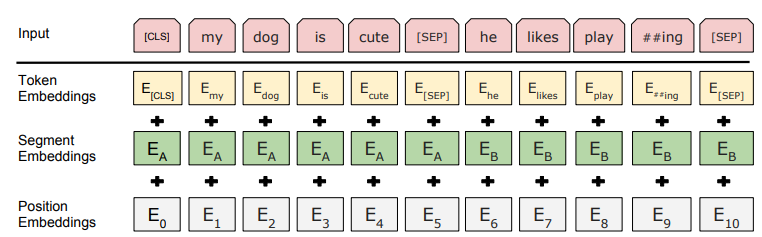
\includegraphics[width=0.75\textwidth]{bert_token.png}
\label{bert_token}
\end{figure}
Для обучения сети без учителя, из входных данных случайно удаляются некоторые члены, их заменяют специальным токеном \textit{[MASK]}. 
\begin{figure}[h]
\caption{Обучение без учителя с масками}
\centering
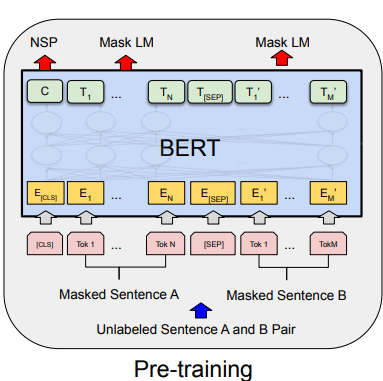
\includegraphics[width=0.5\textwidth]{MLM.png}
\label{mlm}
\end{figure}
Целью сети становится восстановление токенов, сокрытых \textit{[MASK]}, то есть макчимизацией вероятности выбрать правильное слова из словаря на эту позицию. Такой подход позволил обработать большое количество данных без разметки и получить очень сильную модель, которую в процессе тонкой настройки \textit{fine-tuning} можно подготовить для любой задачи в сфере NLP. Очень мощное представление о входных данных будет содержаться в выходном \textit{[CLS]} токене - специальном токене для классификации. Свойства представления данных в нем cхоже с "бутылочным горлышком" в энкодер-декодерных архитектурах.